% VLDB template version of 2020-08-03 enhances the ACM template, version 1.7.0:
% https://www.acm.org/publications/proceedings-template
% The ACM Latex guide provides further information about the ACM template

\documentclass[sigconf, nonacm]{acmart}

%% The following content must be adapted for the final version
% paper-specific
\newcommand\vldbdoi{XX.XX/XXX.XX}
\newcommand\vldbpages{XXX-XXX}
% issue-specific
\newcommand\vldbvolume{14}
\newcommand\vldbissue{1}
\newcommand\vldbyear{2020}
% should be fine as it is
\newcommand\vldbauthors{\authors}
\newcommand\vldbtitle{\shorttitle} 
% leave empty if no availability url should be set
\newcommand\vldbavailabilityurl{https://github.com/moeIsAwesome/repeng-json-schema-extraction}
% whether page numbers should be shown or not, use 'plain' for review versions, 'empty' for camera ready
\newcommand\vldbpagestyle{plain} 

\begin{document}
\title{RepEng Project: An Approach for Schema Extraction of JSON and Extended JSON Document Collections}

%%
%% The "author" command and its associated commands are used to define the authors and their affiliations.

\author{Mohammad Mousavi}
\affiliation{%
  \institution{Universität Passau}
  \city{Passau}
  \country{Germany}
}
\email{mousav03@ads.uni-passau.de}


\maketitle


%%% do not modify the following VLDB block %%
%%% VLDB block start %%%
\ifdefempty{\vldbavailabilityurl}{}{
\vspace{.3cm}
\begingroup\small\noindent\raggedright\textbf{Artifact Availability:}\\
The source code, data, and/or other artifacts have been made available at \url{\vldbavailabilityurl}.
\endgroup
}
%%% VLDB block end %%%

\section{Introduction}

In the scholarly work authored by Frozza et al. ~\cite{frozza2018approach} the authors address the inherent challenges associated with the schemaless characteristics of JSON documents within NoSQL databases. A common feature of NoSQL DB is that they are schemaless, i.e., they allow the storage of data without prior knowledge of their structure ~\cite{sadalage2012nosql}. However, they argue that the lack of a clearly defined schema does not imply a complete absence of a schema.


The paper by Frozza et al. ~\cite{frozza2018approach} introduces an approach called JSON Schema Discovery, which focuses on generating a unified schema from a set of JSON or Extended JSON documents. While emphasiz- ing NoSQL document-oriented databases due to their widespread use, the approach is designed to generate a JSON Schema for any given collection of JSON documents.


The process involves four steps:
\begin{itemize}
    \item (i) generating raw schemas for each document
    \item (ii) grouping these raw schemas
    \item (iii) unifying them
    \item (iv) generating a final JSON Schema.
\end{itemize}
An example of the output generated during the execution of JSON Schema Discovery Step 1 is illustrated in Figure~\ref{fig:rawschema}.


\section{Approach assessment}

Frozza et al. ~\cite{frozza2018approach} undertook three experiments to assess the quality of schemas generated through JSON Schema Discovery. These experiments encompassed:

\begin{itemize}
    \item A) Quality of JSON document mapping for JSON Schema
    \item B) Processing Time Evaluation
    \item C) Comparison with Related Work.
\end{itemize}
In our study, we specifically focus on the third evaluation, in which Frozza et al. ~\cite{frozza2018approach} conducted the experiments on an ASUS K45VM notebook (IntelR Core TM i7 3610QM @ 2.30 GHz and 8GB of RAM).

In light of Frozza et al.'s ~\cite{frozza2018approach} findings, which are detailed in Table~\ref{table1}, we aim to investigate the reproducibility of their results on our system, a MacBook Air with an Apple M1 processor and 8GB of memory. We seek to reproduce their outcomes, considering that we have access to the exact same datasets used in their study.

The central research question guiding our investigation is: To what extent can the results presented by Frozza et al. ~\cite{frozza2018approach} in Table~\ref{table1} be reproduced on our specified system configuration, given the identical datasets?


\begin{figure}
  \centering
  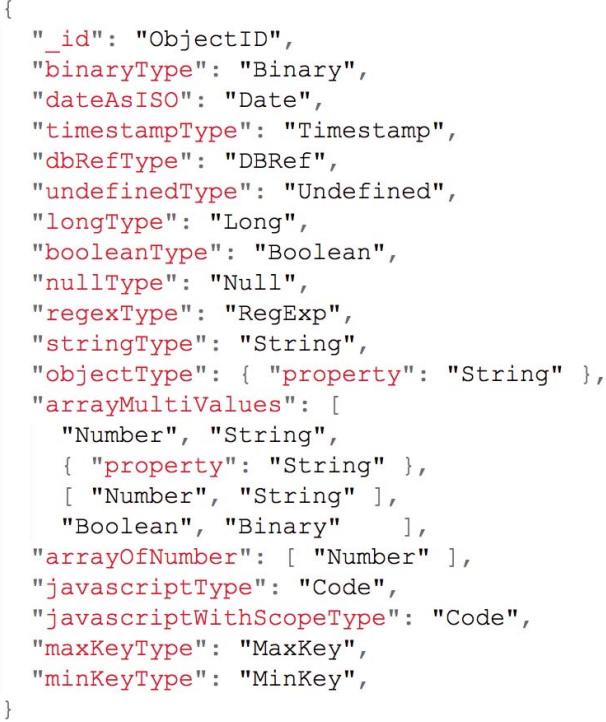
\includegraphics[width=0.6\linewidth]{figures/rawschema.png}
  \vspace{-10pt} % Adjust the value (e.g., 10pt) to your desired spacing
  \caption{Raw schema\cite{frozza2018approach}}
  \label{fig:rawschema}
\end{figure}

\begin{table}[ht]
  \centering
  \caption{Comparison With Wang et al \cite{wang2015schema}}
  \vspace{-10pt}
  \label{tab:example}
  \resizebox{0.4\textwidth}{!}{
    \begin{tabular}{|c|c|c|c|c|}
      \hline
      \multicolumn{2}{|c|}{Datasets} & \multicolumn{2}{|c|}{JSON Schema Discovery} & \multicolumn{1}{|c|}{Wang et al\cite{wang2015schema}} \\
      \hline
      Collection & N\char`_JSON & RS & ROrd & FS\\
      \hline
      drugs & 3662 & 2818 & 2818 & 2818 \\
      \hline
      companies & 24367 & 21312 & 21312 & 21302 \\
      \hline
      movies & 30330 & 25140 & 25140 & 25137 \\
      \hline
    \end{tabular}
  }
  \smallskip
  \vspace{1pt}
  \parbox{0.4\textwidth}{%
    \centering
    \raggedright
    \footnotesize
    N JSON - Number of JSON documents. RS - Raw schemas.\newline ROrd - Raw schemas with ordered structure. TB - Time to obtain the raw schemas. TT - Total time.
  }
        \label{table1}

\end{table}

\subsection{Successful confirmation of results}

To ensure a successful confirmation of result reproduction, a mul- tifaceted approach is employed. Initially, checksums are utilized, incorporating diverse hashing algorithms such as SHA-256 or MD5. This diversified approach minimizes susceptibility to hash collisions, enhancing the robustness of the verification process. Additionally, specialized file differencing tools are employed for a thorough file comparison. Moreover, to facilitate a basic structural consistency check between JSON files, a simple script can be implemented to assess whether the files share identical values at the top level, ensuring a fundamental validation of the data structure’s integrity.



\bibliographystyle{ACM-Reference-Format}
\bibliography{sample}

\end{document}
\endinput